% Task 1 – Khai thác và đặc tả yêu cầu
% Nguồn: docs/requirements/context-and-scope.md, srs.md, use-case-checkout.md
\section{Task 1 -- Khai thác và đặc tả yêu cầu}

%%%%%%%%%%%%%%%%%%%%%%%%%%%%%%%%%%%%%%%%%%%%%%%%%%%%%%%%%%%%%%%%%%%%%%
\subsection{Task 1.1 -- Bối cảnh, stakeholder và phạm vi}\label{sec:context}

\subsubsection{Bối cảnh và vấn đề nghiệp vụ}
BrewLite là một quán cà phê mang đi quy mô nhỏ (một cửa hàng, 2--4 nhân viên quầy). Hiện quán bán theo cách
truyền thống: khách xếp hàng, gọi món bằng lời, nhân viên ghi tay và thu tiền tại quầy. Vào giờ cao điểm
(7:00--9:00 và 11:30--13:00) phát sinh các vấn đề trong Bảng \ref{tab:problems}.

\begin{table}[H]
\centering
\caption{Vấn đề nghiệp vụ hiện tại}\label{tab:problems}
\begin{tabularx}{\textwidth}{|c|X|X|}
\hline
\thead \textbf{\#} & \textbf{Vấn đề hiện tại} & \textbf{Hậu quả} \\ \hline
P1 & Khách phải xếp hàng để gọi món và trả tiền & Thời gian chờ dài, khách bỏ về, mất doanh thu \\ \hline
P2 & Gọi món bằng lời, ghi tay & Sai món, sai size/topping, sai tiền \\ \hline
P3 & Không biết món nào sắp hết & Nhận đơn rồi mới báo hết, khách phàn nàn \\ \hline
P4 & Khách không biết đơn đã xong chưa & Khách đứng chờ quanh quầy, nhân viên bị hỏi liên tục \\ \hline
P5 & Không lưu lịch sử mua hàng & Không chạy được khuyến mãi hay tích điểm để giữ chân khách \\ \hline
P6 & Doanh thu và đơn hàng ghi tay & Quản lý khó đối soát và thống kê \\ \hline
\end{tabularx}
\end{table}

\textbf{Mục tiêu của BrewLite:} cho khách tự xem menu, chọn tùy chọn, đặt và thanh toán trên điện thoại (PWA,
không cần cài ứng dụng từ store), rồi theo dõi trạng thái đơn. Nhân viên nhận đơn đã thanh toán và cập nhật trạng
thái. Quản lý kiểm soát sản phẩm, tồn kho và khuyến mãi.

\begin{table}[H]
\centering
\caption{Mục tiêu đo được}\label{tab:goals}
\begin{tabularx}{\textwidth}{|c|l|X|l|}
\hline
\thead \textbf{Mã} & \textbf{Mục tiêu} & \textbf{Chỉ số} & \textbf{Ngưỡng đạt} \\ \hline
G1 & Giảm thời gian gọi món & Thời gian từ mở app đến thanh toán xong (người dùng mới) & $\le$ 3 phút \\ \hline
G2 & Đơn chính xác & Tỷ lệ đơn sai size/topping so với lựa chọn của khách & 0\% \\ \hline
G3 & Không bán hàng đã hết & Số đơn được tạo khi món đã hết tồn kho & 0 \\ \hline
G4 & Khách biết trạng thái đơn & Thời gian trạng thái mới hiển thị cho khách & $\le$ 5 giây \\ \hline
G5 & Truy cập được để nghiệm thu & URL production HTTPS hoạt động lúc chấm & 100\% \\ \hline
\end{tabularx}
\end{table}

\subsubsection{Stakeholder}

\begin{longtable}{|p{1.1cm}|p{2.0cm}|p{2.3cm}|p{3.1cm}|p{3.8cm}|p{1.5cm}|}
\caption{Bảng stakeholder}\label{tab:stakeholders}\\
\hline
\thead \textbf{Mã} & \textbf{Stakeholder} & \textbf{Vai trò} & \textbf{Mục tiêu} & \textbf{Kỳ vọng với hệ thống} & \textbf{Ảnh hưởng} \\ \hline
\endfirsthead
\hline
\thead \textbf{Mã} & \textbf{Stakeholder} & \textbf{Vai trò} & \textbf{Mục tiêu} & \textbf{Kỳ vọng với hệ thống} & \textbf{Ảnh hưởng} \\ \hline
\endhead
SH-01 & \textbf{Khách hàng} & Người dùng cuối, đặt và trả tiền & Mua đồ uống nhanh, đúng món, không xếp hàng & Menu rõ giá; chọn size/topping dễ; thanh toán Ví/Thẻ nhanh; biết lúc nào đơn xong; xem lại đơn cũ; được khuyến mãi, tích điểm & Trung bình \\ \hline
SH-02 & \textbf{Nhân viên quầy} & Nhận, chế biến đơn, cập nhật trạng thái & Làm đúng món, ít bị hỏi, thao tác nhanh giờ cao điểm & Chỉ thấy đơn đã thanh toán; chi tiết đơn rõ (size, topping, ghi chú); đổi trạng thái một chạm & Trung bình \\ \hline
SH-03 & \textbf{Quản lý cửa hàng} & Chủ nghiệp vụ; quản lý menu, kho, khuyến mãi & Tăng doanh thu, kiểm soát tồn kho, giữ chân khách & Sửa sản phẩm, giá, tồn kho; tạo mã khuyến mãi; xem doanh thu; không bán món đã hết & Cao \\ \hline
SH-04 & \textbf{Giảng viên / khách hàng nghiệm thu} & Đánh giá và nghiệm thu sản phẩm & Kiểm chứng nhóm đi đúng quy trình từ yêu cầu đến triển khai & Tạo phẩm đủ, đúng đường dẫn, truy vết được; CI/CD chạy; URL production hoạt động; clone về chạy được theo README & Rất cao \\ \hline
SH-05 & \textbf{Nhóm phát triển} (1 SV: Phạm Duy Đăng) & Kiêm mọi vai trò: PO, phân tích, thiết kế, lập trình, kiểm thử, triển khai & Hoàn thành đúng hạn, học quy trình chuẩn & Yêu cầu rõ ràng, ổn định; stack bắt buộc; hạ tầng miễn phí & Cao \\ \hline
SH-06 & \textbf{Đơn vị thanh toán} (mô phỏng) & Hệ thống ngoài xử lý giao dịch Ví/Thẻ & Giao dịch hợp lệ, không trừ tiền trùng & API rõ ràng; mỗi giao dịch có idempotency key; trả kết quả kèm mã lỗi; không nhận dữ liệu thẻ thừa & Trung bình \\ \hline
\end{longtable}

\begin{table}[H]
\centering
\caption{Ma trận quyền lực -- quan tâm}\label{tab:power}
\begin{tabularx}{\textwidth}{|l|X|X|}
\hline
\thead & \textbf{Quan tâm thấp} & \textbf{Quan tâm cao} \\ \hline
\textbf{Ảnh hưởng cao} & -- & SH-03, SH-04, SH-05: quản lý chặt, duyệt mọi thay đổi phạm vi \\ \hline
\textbf{Ảnh hưởng thấp/TB} & SH-06: theo dõi, tuân thủ hợp đồng API & SH-01, SH-02: cập nhật thường xuyên, thử nghiệm khả dụng \\ \hline
\end{tabularx}
\end{table}

\subsubsection{Phạm vi}

\begin{table}[H]
\centering
\caption{Phạm vi MVP (in-scope, Must)}\label{tab:inscope}
\begin{tabularx}{\textwidth}{|c|X|l|}
\hline
\thead \textbf{\#} & \textbf{Hạng mục} & \textbf{Yêu cầu} \\ \hline
S1 & Xem menu theo danh mục, có trạng thái loading/empty/error & FR-01 \\ \hline
S2 & Chi tiết sản phẩm: chọn size và topping, giá cập nhật theo lựa chọn & FR-02 \\ \hline
S3 & Giỏ hàng và tính tổng tiền & FR-03 \\ \hline
S4 & Đặt đơn: kiểm tra và trừ tồn kho trong một transaction & FR-04 \\ \hline
S5 & Thanh toán Ví/Thẻ qua dịch vụ thanh toán mô phỏng & FR-05 \\ \hline
S6 & Idempotency khi client gửi lại yêu cầu thanh toán & FR-06 \\ \hline
S7 & Xác nhận và theo dõi trạng thái đơn & FR-07 \\ \hline
S8 & Lịch sử đơn của khách & FR-08 \\ \hline
S9 & Đăng ký, đăng nhập/đăng xuất bằng JWT & FR-09, FR-10 \\ \hline
S10 & Phân quyền Khách hàng / Nhân viên / Quản lý & FR-11 \\ \hline
S11 & Nhân viên cập nhật trạng thái đơn & FR-12 \\ \hline
S12 & PWA mobile-first, health check, Docker Compose, CI/CD, production HTTPS & NFR-09, 11, 14--17 \\ \hline
\end{tabularx}
\end{table}

\begin{table}[H]
\centering
\caption{Phạm vi mở rộng (Should/Could)}\label{tab:extscope}
\begin{tabularx}{\textwidth}{|c|X|c|l|}
\hline
\thead \textbf{\#} & \textbf{Hạng mục} & \textbf{Ưu tiên} & \textbf{Yêu cầu} \\ \hline
E1 & Hủy đơn chưa thanh toán, tự hủy đơn quá hạn 15 phút, hoàn lại tồn kho & Should & FR-13 \\ \hline
E2 & Áp mã khuyến mãi (Promotion) & Should & FR-14 \\ \hline
E3 & Tích điểm thành viên (LoyaltyTransaction) & Should & FR-15 \\ \hline
E4 & Quản lý sản phẩm và tồn kho cho Quản lý & Should & FR-16 \\ \hline
E5 & Tìm kiếm, lọc menu & Should & FR-17 \\ \hline
E6 & Dùng điểm để giảm giá & Could & FR-18 \\ \hline
E7 & Báo cáo doanh thu theo ngày & Could & FR-19 \\ \hline
E8 & Thông báo đẩy (Web Push) khi đơn sẵn sàng & Could & FR-20 \\ \hline
\end{tabularx}
\end{table}

\begin{table}[H]
\centering
\caption{Ngoài phạm vi (out-of-scope, Won't)}\label{tab:outscope}
\begin{tabularx}{\textwidth}{|c|l|X|}
\hline
\thead \textbf{\#} & \textbf{Nội dung} & \textbf{Lý do} \\ \hline
O1 & Cổng thanh toán thật (VNPay, MoMo, Stripe\dots) & Đề bài yêu cầu mô phỏng; cần hợp đồng và tài khoản merchant (FR-21) \\ \hline
O2 & Giao hàng tận nơi & Ngoài nghiệp vụ quán mang đi (FR-22) \\ \hline
O3 & Nhiều chi nhánh & Quán chỉ có một cửa hàng (FR-23) \\ \hline
O4 & Đăng nhập Google/Facebook & Không cần cho MVP, tăng rủi ro cấu hình OAuth (FR-24) \\ \hline
O5 & Ứng dụng native iOS/Android & Đã có PWA thay thế \\ \hline
O6 & Quản lý nguyên liệu & Tồn kho chỉ tính theo số ly của từng sản phẩm \\ \hline
O7 & Hoàn tiền tự động & Đơn chỉ hủy được khi chưa thanh toán \\ \hline
O8 & Hạ tầng đa vùng, sẵn sàng cao & Vượt nguồn lực của đồ án (NFR-20) \\ \hline
\end{tabularx}
\end{table}

\subsubsection{Giả định và ràng buộc}

\begin{table}[H]
\centering
\caption{Giả định}\label{tab:assumptions}
\begin{tabularx}{\textwidth}{|c|X|}
\hline
\thead \textbf{Mã} & \textbf{Giả định} \\ \hline
A1 & Quán có một cửa hàng; mọi đơn là mang đi hoặc dùng tại quán, khách tự đến quầy nhận. \\ \hline
A2 & Khách có smartphone, trình duyệt hiện đại (Chrome Android, Safari iOS) và có Internet khi đặt đơn. \\ \hline
A3 & Tiền tệ là VND, số nguyên, giá đã gồm VAT. \\ \hline
A4 & Tồn kho tính theo sản phẩm (số ly còn bán được). Size và topping không có tồn kho riêng. \\ \hline
A5 & Đơn vị thanh toán là dịch vụ mô phỏng, trả kết quả theo bộ dữ liệu test cố định. Không có tiền thật. \\ \hline
A6 & Khách phải đăng nhập mới đặt đơn được. Khách vãng lai chỉ xem menu, chi tiết sản phẩm và giỏ hàng. \\ \hline
A7 & Tài khoản Nhân viên và Quản lý được tạo sẵn bằng seed hoặc do Quản lý tạo. \\ \hline
A8 & Đơn chưa thanh toán giữ tồn kho tối đa 15 phút, sau đó tự hủy và trả lại tồn kho. \\ \hline
A9 & Nhóm dùng gói miễn phí của các nền tảng cloud; cold start vài giây ở lần gọi đầu là chấp nhận được. \\ \hline
\end{tabularx}
\end{table}

\begin{longtable}{|c|l|p{11.5cm}|}
\caption{Ràng buộc}\label{tab:constraints}\\
\hline
\thead \textbf{Mã} & \textbf{Loại} & \textbf{Ràng buộc} \\ \hline
\endfirsthead
\hline
\thead \textbf{Mã} & \textbf{Loại} & \textbf{Ràng buộc} \\ \hline
\endhead
C1 & Công nghệ & Bắt buộc Next.js (mobile-first/PWA), NestJS và PostgreSQL. Được bổ sung nhưng không được thay thế. \\ \hline
C2 & Công nghệ & Đóng gói bằng Docker; \code{docker-compose.yml} chạy web, API và DB ở local. \\ \hline
C3 & Quy trình & 5 task làm tuần tự; tạo phẩm mỗi task phải có trên repo với lịch sử commit/PR rõ ràng. \\ \hline
C4 & Quy trình & Mọi thay đổi yêu cầu, sơ đồ hoặc kiến trúc phải đi qua commit/PR và ghi lý do. \\ \hline
C5 & Quy trình & Pull request không được merge nếu lint, test hoặc build thất bại. \\ \hline
C6 & Cấu trúc & Repo theo cấu trúc \code{apps/web}, \code{apps/api}, \code{docs/}, \code{tests/}, \code{.github/workflows/}. \\ \hline
C7 & Triển khai & Production có HTTPS; database không public; secret không nằm trong repo hay log CI. \\ \hline
C8 & Thời gian & Hai Sprint trong học kỳ I 2026--2027; production phải hoạt động lúc chấm. \\ \hline
C9 & Chi phí & 0 đồng: chỉ dùng gói miễn phí (GitHub, GHCR, Vercel/Render/Neon hoặc tương đương). \\ \hline
C10 & Pháp lý & Không lưu số thẻ đầy đủ hay CVV, kể cả dữ liệu mô phỏng; chỉ lưu 4 số cuối. \\ \hline
C11 & Nhân lực & Đề tài do một sinh viên thực hiện, kiêm toàn bộ vai trò; không có người review chéo trong nhóm. \\ \hline
\end{longtable}

\subsubsection{Rủi ro ban đầu}
Thang đo xác suất (X) và tác động (T) từ 1 (thấp) đến 3 (cao); Điểm = X $\times$ T.

\begin{longtable}{|c|p{4.3cm}|c|c|c|p{6.2cm}|}
\caption{Rủi ro ban đầu}\label{tab:risks}\\
\hline
\thead \textbf{Mã} & \textbf{Rủi ro} & \textbf{X} & \textbf{T} & \textbf{Điểm} & \textbf{Biện pháp giảm thiểu} \\ \hline
\endfirsthead
\hline
\thead \textbf{Mã} & \textbf{Rủi ro} & \textbf{X} & \textbf{T} & \textbf{Điểm} & \textbf{Biện pháp giảm thiểu} \\ \hline
\endhead
R1 & Nền tảng miễn phí hết hạn hoặc ngủ đúng lúc chấm & 2 & 3 & \textbf{6} & Dùng Postgres không hết hạn (Neon); smoke test định kỳ; quy trình redeploy và rollback sẵn \\ \hline
R2 & Bán vượt tồn kho khi nhiều khách đặt cùng lúc & 2 & 3 & \textbf{6} & Trừ kho có điều kiện \code{stock >= qty} trong transaction; test đồng thời (NFR-13) \\ \hline
R3 & Trừ tiền hai lần khi khách bấm lại hoặc mạng chập chờn & 2 & 3 & \textbf{6} & Idempotency key cho mỗi yêu cầu thanh toán; tối đa 1 payment thành công mỗi đơn (FR-06) \\ \hline
R4 & Phạm vi phình to làm trễ luồng chính & 3 & 2 & \textbf{6} & Ưu tiên MoSCoW; làm Must trước, Should/Could sau khi luồng end-to-end chạy \\ \hline
R5 & Chưa quen NestJS, Docker, CI/CD & 2 & 2 & 4 & Dựng khung và CI từ Sprint 1; làm theo tài liệu chính thức; ghi lại trong README \\ \hline
R6 & Lộ secret lên GitHub & 1 & 3 & 3 & \code{.env} trong \code{.gitignore}; chỉ commit \code{.env.example}; GitHub Secrets; quét secret trong CI \\ \hline
R7 & Tài liệu và code lệch nhau & 2 & 2 & 4 & Ma trận truy vết; mọi thay đổi yêu cầu qua PR \\ \hline
R8 & Cold start làm smoke test hoặc demo chậm & 2 & 1 & 2 & Smoke test có retry; ``đánh thức'' dịch vụ trước demo \\ \hline
R9 & Một người làm toàn bộ: quá tải, không ai review chéo & 2 & 3 & \textbf{6} & Cắt phạm vi theo MoSCoW; CI tự động thay review chéo; mọi thay đổi qua PR có checklist \\ \hline
\end{longtable}

%%%%%%%%%%%%%%%%%%%%%%%%%%%%%%%%%%%%%%%%%%%%%%%%%%%%%%%%%%%%%%%%%%%%%%
\newpage
\subsection{Task 1.2 -- Yêu cầu chức năng và phi chức năng (SRS)}\label{sec:srs}

\subsubsection{Quy ước}
Mỗi yêu cầu có mã định danh duy nhất (\code{FR-xx}, \code{NFR-xx}), mức ưu tiên MoSCoW và tiêu chí chấp nhận
kiểm chứng được, đánh mã \code{AC-xx.y}. Test ở các task sau tham chiếu trực tiếp tới mã AC.

\begin{table}[H]
\centering
\caption{Quy ước MoSCoW}\label{tab:moscow}
\begin{tabularx}{\textwidth}{|l|X|}
\hline
\thead \textbf{Mức} & \textbf{Ý nghĩa trong dự án} \\ \hline
\textbf{Must} & Bắt buộc cho MVP; thiếu thì luồng end-to-end không chạy hoặc không đạt yêu cầu đề bài. \\ \hline
\textbf{Should} & Quan trọng, làm trong Sprint 2 sau khi các Must đã chạy end-to-end. \\ \hline
\textbf{Could} & Làm nếu còn thời gian; không ảnh hưởng nghiệm thu. \\ \hline
\textbf{Won't} & Đã thống nhất không làm trong phiên bản này; ghi lại để tránh phình phạm vi. \\ \hline
\end{tabularx}
\end{table}

Quy ước chung: tiền tệ VND số nguyên (hiển thị \code{45.000 đ}); mọi API có tiền tố \code{/api/v1}; lỗi API
trả JSON thống nhất \code{\{ statusCode, code, message, details \}}; thời gian lưu UTC, hiển thị theo
\code{Asia/Ho\_Chi\_Minh}.

\subsubsection{Tác nhân và vai trò}

\begin{table}[H]
\centering
\caption{Tác nhân}\label{tab:actors}
\begin{tabularx}{\textwidth}{|l|l|X|c|}
\hline
\thead \textbf{Tác nhân} & \textbf{Vai trò} & \textbf{Mô tả} & \textbf{Stakeholder} \\ \hline
Khách vãng lai & -- & Chưa đăng nhập; xem menu, chi tiết sản phẩm, giỏ hàng & SH-01 \\ \hline
Khách hàng & \code{CUSTOMER} & Kế thừa Khách vãng lai; đặt đơn, thanh toán, xem đơn của mình, tích điểm & SH-01 \\ \hline
Nhân viên quầy & \code{STAFF} & Xem đơn đã thanh toán, cập nhật trạng thái chế biến & SH-02 \\ \hline
Quản lý cửa hàng & \code{MANAGER} & Kế thừa Nhân viên; quản lý sản phẩm, tồn kho, khuyến mãi, báo cáo & SH-03 \\ \hline
Payment Service & Hệ thống ngoài & Dịch vụ thanh toán mô phỏng xử lý giao dịch Ví/Thẻ & SH-06 \\ \hline
Bộ hẹn giờ & Hệ thống nội bộ & Tác vụ định kỳ hủy đơn quá hạn thanh toán & -- \\ \hline
\end{tabularx}
\end{table}

\subsubsection{Quy tắc nghiệp vụ}

\begin{longtable}{|c|p{14.2cm}|}
\caption{Quy tắc nghiệp vụ}\label{tab:br}\\
\hline
\thead \textbf{Mã} & \textbf{Quy tắc} \\ \hline
\endfirsthead
\hline
\thead \textbf{Mã} & \textbf{Quy tắc} \\ \hline
\endhead
BR-01 & Mỗi sản phẩm có giá cơ bản (\code{basePrice}), danh sách size kèm phụ thu (mặc định S +0, M +5.000, L +10.000; cấu hình được theo sản phẩm) và danh sách topping kèm giá. \\ \hline
BR-02 & Thành tiền một dòng = (\code{basePrice} + phụ thu size + $\Sigma$ giá topping) $\times$ số lượng. \\ \hline
BR-03 & Mỗi dòng chọn đúng 1 size và 0--3 topping khác nhau; số lượng mỗi dòng 1--10; một đơn tối đa 20 ly; ghi chú mỗi dòng $\le$ 100 ký tự. \\ \hline
BR-04 & Tạm tính = $\Sigma$ thành tiền các dòng. Giảm giá = khuyến mãi (BR-13) + đổi điểm (BR-15). Tổng = Tạm tính $-$ Giảm giá, luôn $\ge$ 0. \\ \hline
BR-05 & Server luôn tự tính lại giá từ database, bỏ qua giá client gửi. Lệch \code{expectedTotal} thì trả 409 \code{PRICE\_CHANGED} kèm giá mới. \\ \hline
BR-06 & Khi tạo đơn, tên và đơn giá của sản phẩm, size, topping được chụp lại (snapshot) vào \code{OrderItem}; sửa menu về sau không đổi đơn cũ. \\ \hline
BR-07 & Tồn kho được kiểm tra và trừ trong cùng transaction với việc tạo đơn. Một món không đủ thì cả đơn bị từ chối (409 \code{OUT\_OF\_STOCK}) và không món nào bị trừ. Tồn kho không bao giờ âm. \\ \hline
BR-08 & Đơn \code{PENDING\_PAYMENT} quá 15 phút (\code{expiresAt}) bị hủy tự động và hoàn lại tồn kho. \\ \hline
BR-09 & Mỗi đơn được thanh toán thất bại tối đa 3 lần; lần thứ 3 làm đơn chuyển \code{CANCELLED} và hoàn kho. \\ \hline
BR-10 & Mỗi đơn có tối đa 1 payment \code{SUCCEEDED}; số tiền thanh toán luôn bằng \code{Order.total}. \\ \hline
BR-11 & Mỗi yêu cầu thanh toán kèm header \code{Idempotency-Key} (UUID v4), hiệu lực 24 giờ trong phạm vi một người dùng. Cùng khóa, cùng nội dung: trả đúng kết quả cũ và không gọi Payment Service lần hai. Cùng khóa, khác nội dung: 422 \code{IDEMPOTENCY\_KEY\_REUSED}. \\ \hline
BR-12 & Luồng trạng thái hợp lệ: \code{PENDING\_PAYMENT} $\rightarrow$ \code{PAID}; \code{PENDING\_PAYMENT} $\rightarrow$ \code{CANCELLED}; \code{PAID} $\rightarrow$ \code{PREPARING} $\rightarrow$ \code{READY} $\rightarrow$ \code{COMPLETED}. Mọi chuyển khác bị từ chối; không hủy được đơn đã \code{PAID}. \\ \hline
BR-13 & Mã khuyến mãi hợp lệ khi đang bật, trong thời hạn, \code{usedCount < usageLimit} và Tạm tính $\ge$ \code{minOrderValue}. Loại \code{PERCENT} có trần \code{maxDiscount}; loại \code{FIXED} không vượt Tạm tính. Mỗi đơn tối đa 1 mã; \code{usedCount} chỉ tăng khi đơn \code{PAID}. \\ \hline
BR-14 & Khi đơn chuyển \code{PAID}, khách được \code{floor(Tổng / 10.000)} điểm; mỗi đơn chỉ cộng điểm một lần. \\ \hline
BR-15 & Đổi điểm (Could): 1 điểm = 1.000 đ, tối đa 50\% Tạm tính sau khuyến mãi; điểm bị trừ khi đơn \code{PAID}. \\ \hline
BR-16 & Mã đơn dạng \code{BL-YYMMDD-NNNN}; \code{NNNN} tăng dần trong ngày và là số gọi món ở quầy. \\ \hline
BR-17 & Khách chỉ xem và thao tác được đơn của chính mình; truy cập đơn người khác trả 404. \\ \hline
BR-18 & Không lưu số thẻ đầy đủ và CVV; database chỉ lưu \code{cardLast4} và \code{cardBrand}. \\ \hline
\end{longtable}

\begin{table}[H]
\centering
\caption{Dữ liệu test của Payment Service mô phỏng}\label{tab:paytest}
\begin{tabularx}{\textwidth}{|l|l|X|l|}
\hline
\thead \textbf{Phương thức} & \textbf{Dữ liệu test} & \textbf{Kết quả} & \textbf{Mã lỗi} \\ \hline
Thẻ & \code{4242 4242 4242 4242} & Thành công & -- \\ \hline
Thẻ & \code{4000 0000 0000 0002} & Thất bại & \code{CARD\_DECLINED} \\ \hline
Thẻ & \code{4000 0000 0000 9995} & Thất bại & \code{INSUFFICIENT\_FUNDS} \\ \hline
Thẻ & \code{4000 0000 0000 0119} & Lần đầu chậm hơn 10 giây (timeout); gửi lại cùng khóa thì thành công & \code{PAYMENT\_TIMEOUT} \\ \hline
Thẻ & Số thẻ hợp lệ Luhn khác & Thành công & -- \\ \hline
Ví & SĐT \code{0900000001} & Thất bại & \code{INSUFFICIENT\_FUNDS} \\ \hline
Ví & SĐT \code{0900000002} & Thất bại & \code{WALLET\_LOCKED} \\ \hline
Ví & SĐT di động hợp lệ khác & Thành công & -- \\ \hline
\end{tabularx}
\end{table}

\subsubsection{Yêu cầu chức năng}

\begin{longtable}{|c|l|p{5.5cm}|c|c|c|}
\caption{Tổng hợp yêu cầu chức năng}\label{tab:fr}\\
\hline
\thead \textbf{Mã} & \textbf{Nhóm} & \textbf{Tên yêu cầu} & \textbf{Ưu tiên} & \textbf{Sprint} & \textbf{UC} \\ \hline
\endfirsthead
\hline
\thead \textbf{Mã} & \textbf{Nhóm} & \textbf{Tên yêu cầu} & \textbf{Ưu tiên} & \textbf{Sprint} & \textbf{UC} \\ \hline
\endhead
FR-01 & Menu & Xem menu & Must & 1 & UC-02 \\ \hline
FR-02 & Chi tiết sản phẩm & Xem chi tiết, chọn size và topping & Must & 1/2 & UC-02 \\ \hline
FR-03 & Giỏ hàng & Quản lý giỏ hàng, tính tổng tiền & Must & 2 & UC-03 \\ \hline
FR-04 & Đặt đơn & Tạo đơn, kiểm tra và trừ tồn kho & Must & 2 & UC-01 \\ \hline
FR-05 & Thanh toán & Thanh toán Ví/Thẻ mô phỏng & Must & 2 & UC-01, 14 \\ \hline
FR-06 & Thanh toán & Idempotency khi gửi lại yêu cầu thanh toán & Must & 2 & UC-01 \\ \hline
FR-07 & Trạng thái đơn & Xác nhận và theo dõi trạng thái đơn & Must & 2 & UC-06 \\ \hline
FR-08 & Lịch sử đơn & Xem lịch sử đơn & Must & 2 & UC-07 \\ \hline
FR-09 & Xác thực & Đăng ký tài khoản khách hàng & Must & 2 & UC-04 \\ \hline
FR-10 & Xác thực & Đăng nhập, đăng xuất bằng JWT & Must & 2 & UC-05 \\ \hline
FR-11 & Xác thực & Phân quyền theo vai trò & Must & 2 & Tất cả \\ \hline
FR-12 & Quản lý trạng thái & Nhân viên cập nhật trạng thái đơn & Must & 2 & UC-10 \\ \hline
FR-13 & Đặt đơn & Hủy đơn chưa thanh toán, tự hủy đơn quá hạn & Should & 2 & UC-12, 15 \\ \hline
FR-14 & Khuyến mãi & Áp dụng mã khuyến mãi & Should & 2 & UC-08 \\ \hline
FR-15 & Loyalty & Tích điểm thành viên & Should & 2 & UC-09 \\ \hline
FR-16 & Quản trị & Quản lý sản phẩm và tồn kho & Should & 2 & UC-11 \\ \hline
FR-17 & Menu & Tìm kiếm và lọc menu & Should & 2 & UC-02 \\ \hline
FR-18 & Loyalty & Đổi điểm lấy giảm giá & Could & -- & UC-09 \\ \hline
FR-19 & Quản trị & Báo cáo doanh thu theo ngày & Could & -- & UC-13 \\ \hline
FR-20 & Thông báo & Thông báo đẩy khi đơn sẵn sàng & Could & -- & UC-06 \\ \hline
FR-21 & Thanh toán & Tích hợp cổng thanh toán thật & Won't & -- & -- \\ \hline
FR-22 & Đặt đơn & Giao hàng tận nơi & Won't & -- & -- \\ \hline
FR-23 & Quản trị & Quản lý nhiều chi nhánh & Won't & -- & -- \\ \hline
FR-24 & Xác thực & Đăng nhập bằng mạng xã hội & Won't & -- & -- \\ \hline
\end{longtable}

\paragraph{Tiêu chí chấp nhận chi tiết}\mbox{}

\begin{description}[style=nextline,leftmargin=1.6cm,labelwidth=1.4cm,font=\normalfont\ttfamily]

\item[] \textbf{FR-01 -- Xem menu (Must)}
\item[AC-01.1] \code{GET /products} trả 200, không cần token, mảng sản phẩm \code{isActive = true}; mỗi phần tử có \code{id}, \code{name}, \code{imageUrl}, \code{basePrice}, \code{category}, \code{inStock} (= \code{stock > 0}).
\item[AC-01.2] Không trả sản phẩm \code{isActive = false}.
\item[AC-01.3] Màn menu hiện skeleton khi tải; ``Chưa có món nào'' khi rỗng; thông báo lỗi và nút ``Thử lại'' khi API lỗi hoặc mất mạng.
\item[AC-01.4] Sản phẩm \code{inStock = false} hiện nhãn ``Hết hàng'' và không có nút thêm vào giỏ.
\item[AC-01.5] Ở chiều rộng 360 px trang không cuộn ngang, mỗi sản phẩm hiện đủ ảnh, tên, giá.

\item[] \textbf{FR-02 -- Xem chi tiết sản phẩm, chọn size và topping (Must)}
\item[AC-02.1] \code{GET /products/:id} trả 200 với thông tin FR-01, thêm \code{description}, \code{sizes[]}, \code{toppings[]}.
\item[AC-02.2] \code{id} không tồn tại hoặc sản phẩm ngừng bán: 404 \code{PRODUCT\_NOT\_FOUND}; \code{id} sai định dạng UUID: 400.
\item[AC-02.3] Màn chi tiết chọn sẵn size đầu tiên; chỉ chọn được đúng 1 size.
\item[AC-02.4] Chọn được 0--3 topping; đủ 3 thì các topping còn lại bị vô hiệu hóa.
\item[AC-02.5] Giá cập nhật ngay khi đổi size, topping, số lượng, đúng BR-02. Ví dụ: basePrice 35.000, size L (+10.000), trân châu 5.000, số lượng 2 $\rightarrow$ 100.000 đ.
\item[AC-02.6] Số lượng chỉ 1--10; ghi chú quá 100 ký tự thì báo lỗi và vô hiệu nút ``Thêm vào giỏ''.

\item[] \textbf{FR-03 -- Quản lý giỏ hàng và tính tổng tiền (Must)}
\item[AC-03.1] ``Thêm vào giỏ'' làm giỏ tăng đúng số lượng, biểu tượng giỏ cập nhật số ly.
\item[AC-03.2] Cùng sản phẩm, size, bộ topping và ghi chú thì gộp một dòng; khác bất kỳ yếu tố nào thì tạo dòng mới.
\item[AC-03.3] Sửa số lượng (1--10), xóa từng dòng; thành tiền và Tạm tính cập nhật đúng BR-02, BR-04.
\item[AC-03.4] Giỏ giữ nguyên sau khi tải lại trang và sau khi đăng nhập.
\item[AC-03.5] Khách vãng lai dùng được giỏ hàng.
\item[AC-03.6] Giỏ rỗng hiện ``Giỏ hàng trống'', nút ``Đặt hàng'' bị vô hiệu hóa.
\item[AC-03.7] Thao tác làm tổng số ly vượt 20 thì không thực hiện và hiện thông báo.

\item[] \textbf{FR-04 -- Tạo đơn, kiểm tra và trừ tồn kho (Must)}
\item[AC-04.1] \code{POST /orders} không có JWT hợp lệ: 401; giao diện chuyển đăng nhập, giữ giỏ, quay lại thanh toán sau khi đăng nhập.
\item[AC-04.2] Body sai định dạng: 400 kèm lỗi từng trường; không tạo đơn.
\item[AC-04.3] Server tự tính lại giá (BR-05); lệch \code{expectedTotal}: 409 \code{PRICE\_CHANGED}.
\item[AC-04.4] Thành công: 201 với \code{id}, \code{code}, \code{status = PENDING\_PAYMENT}, \code{subtotal}, \code{discount}, \code{total}, \code{expiresAt}; tồn kho giảm đúng số lượng đặt.
\item[AC-04.5] Một món không đủ tồn kho: 409 \code{OUT\_OF\_STOCK} kèm \code{productIds}; tồn kho mọi sản phẩm giữ nguyên, không có đơn.
\item[AC-04.6] Đặt món đã ngừng bán: 409 \code{PRODUCT\_UNAVAILABLE}.
\item[AC-04.7] Đơn lưu snapshot (BR-06); sửa giá sau khi đặt không đổi \code{total} của đơn.
\item[AC-04.8] Tạo đơn thành công thì giỏ được xóa và giao diện chuyển sang bước thanh toán.

\item[] \textbf{FR-05 -- Thanh toán Ví/Thẻ mô phỏng (Must)}
\item[AC-05.1] \code{POST /payments} \code{\{orderId, method, card?, wallet?\}} yêu cầu JWT; chỉ chủ đơn gọi được, người khác nhận 404.
\item[AC-05.2] FE và BE cùng kiểm tra: số thẻ đúng Luhn, 16 chữ số; hạn chưa qua; CVV 3 chữ số; SĐT ví 10 chữ số. Sai: 400 và không gọi Payment Service.
\item[AC-05.3] Đơn không ở \code{PENDING\_PAYMENT} hoặc đã quá hạn: 409 \code{ORDER\_NOT\_PAYABLE}.
\item[AC-05.4] Thành công: 201 \code{\{paymentId, status: SUCCEEDED, orderStatus: PAID\}}; \code{Payment.amount = Order.total}.
\item[AC-05.5] Thất bại: 402 \code{PAYMENT\_FAILED} kèm lý do; Payment \code{FAILED}, đơn vẫn \code{PENDING\_PAYMENT}; giao diện cho thử lại hoặc đổi phương thức.
\item[AC-05.6] Thất bại lần thứ 3: đơn \code{CANCELLED}, tồn kho được hoàn (BR-09).
\item[AC-05.7] Payment Service không phản hồi trong 10 giây: 202 \code{\{status: PENDING\}}; giao diện tự gửi lại cùng \code{Idempotency-Key}.
\item[AC-05.8] Bảng \code{payments} và log không chứa số thẻ đầy đủ hay CVV; chỉ có \code{cardLast4}, \code{cardBrand}.

\item[] \textbf{FR-06 -- Idempotency khi gửi lại yêu cầu thanh toán (Must)}
\item[AC-06.1] Thiếu header \code{Idempotency-Key} hoặc không phải UUID: 400.
\item[AC-06.2] Cùng khóa, cùng body trong 24 giờ: cùng mã HTTP và body; Payment Service được gọi đúng 1 lần.
\item[AC-06.3] Cùng khóa, khác body: 422 \code{IDEMPOTENCY\_KEY\_REUSED}.
\item[AC-06.4] Hai request đồng thời cùng khóa: chỉ một được xử lý, request còn lại nhận cùng kết quả hoặc 409 \code{REQUEST\_IN\_PROGRESS}.
\item[AC-06.5] Đơn đã \code{PAID} nhận khóa mới: 409 \code{ORDER\_ALREADY\_PAID}; không bao giờ có 2 payment \code{SUCCEEDED} cho một đơn.

\item[] \textbf{FR-07 -- Xác nhận và theo dõi trạng thái đơn (Must)}
\item[AC-07.1] Thanh toán thành công thì chuyển tới \code{/orders/:id}: mã đơn, số gọi món, món, tổng tiền, phương thức (thẻ hiện 4 số cuối), trạng thái.
\item[AC-07.2] \code{GET /orders/:id} chỉ trả cho chủ đơn, Staff, Manager; người khác nhận 404.
\item[AC-07.3] Nhân viên đổi trạng thái thì khách thấy trạng thái mới trong $\le$ 5 giây, không cần tải lại trang.
\item[AC-07.4] Có dòng thời gian các trạng thái đã qua kèm giờ, phút.

\item[] \textbf{FR-08 -- Xem lịch sử đơn (Must)}
\item[AC-08.1] \code{GET /orders?page=1\&limit=10} yêu cầu JWT, chỉ trả đơn của người gọi, mới nhất trước, mặc định 10 đơn/trang.
\item[AC-08.2] Mỗi dòng hiện mã đơn, ngày giờ, số ly, tổng tiền, trạng thái; bấm vào mở chi tiết.
\item[AC-08.3] Chưa có đơn: hiện ``Bạn chưa có đơn nào'' và nút ``Xem menu''.

\item[] \textbf{FR-09 -- Đăng ký tài khoản khách hàng (Must)}
\item[AC-09.1] \code{POST /auth/register} với \code{email}, \code{password}, \code{fullName}, \code{phone?}: 201; tài khoản vai trò \code{CUSTOMER}, 0 điểm.
\item[AC-09.2] FE và BE kiểm tra: email hợp lệ; mật khẩu $\ge$ 8 ký tự có chữ và số; họ tên 2--50 ký tự; SĐT 10 chữ số. Sai: 400.
\item[AC-09.3] Email đã tồn tại (không phân biệt hoa thường): 409 \code{EMAIL\_TAKEN}.
\item[AC-09.4] Mật khẩu lưu hash bcrypt; không response nào chứa mật khẩu hay hash.

\item[] \textbf{FR-10 -- Đăng nhập, đăng xuất bằng JWT (Must)}
\item[AC-10.1] \code{POST /auth/login} đúng: 200 \code{\{accessToken, expiresIn: 3600, user\}}.
\item[AC-10.2] Sai email hoặc mật khẩu đều trả 401 \code{INVALID\_CREDENTIALS} cùng thông báo.
\item[AC-10.3] Endpoint cần đăng nhập trả 401 khi token thiếu, sai chữ ký hoặc hết hạn (60 phút).
\item[AC-10.4] Đăng xuất xóa token phía client và chuyển về menu.
\item[AC-10.5] Token hết hạn giữa chừng: chuyển đăng nhập kèm \code{returnUrl}, không mất giỏ hàng.

\item[] \textbf{FR-11 -- Phân quyền theo vai trò (Must)}
\item[AC-11.1] Ba vai trò \code{CUSTOMER}, \code{STAFF}, \code{MANAGER} nằm trong claim \code{role} của JWT và được kiểm tra ở server.
\item[AC-11.2] \code{CUSTOMER} gọi \code{/staff/*} hoặc \code{/manager/*}: 403; \code{STAFF} gọi \code{/manager/*}: 403.
\item[AC-11.3] \code{MANAGER} gọi được mọi endpoint của \code{STAFF}.
\item[AC-11.4] Giao diện ẩn menu không thuộc vai trò; truy cập thẳng URL vẫn bị server chặn.

\item[] \textbf{FR-12 -- Nhân viên cập nhật trạng thái đơn (Must)}
\item[AC-12.1] \code{GET /staff/orders} trả đơn \code{PAID}, \code{PREPARING}, \code{READY}, cũ nhất trước; không trả đơn \code{PENDING\_PAYMENT}.
\item[AC-12.2] Màn nhân viên có 3 cột Đã thanh toán -- Đang pha -- Sẵn sàng; đơn mới xuất hiện trong $\le$ 5 giây.
\item[AC-12.3] \code{PATCH /staff/orders/:id/status} chỉ chấp nhận chuyển đúng BR-12; sai: 409 \code{INVALID\_TRANSITION}.
\item[AC-12.4] Mỗi lần chuyển trạng thái ghi lịch sử: trạng thái cũ, mới, người thực hiện, thời điểm.

\item[] \textbf{FR-13 -- Hủy đơn chưa thanh toán và tự hủy đơn quá hạn (Should)}
\item[AC-13.1] \code{POST /orders/:id/cancel} khi đơn \code{PENDING\_PAYMENT}: đơn \code{CANCELLED} và hoàn kho trong cùng transaction.
\item[AC-13.2] Hủy đơn ở trạng thái khác: 409 \code{ORDER\_NOT\_CANCELLABLE}.
\item[AC-13.3] Tác vụ định kỳ chạy mỗi phút hủy đơn quá \code{expiresAt} và hoàn kho.

\item[] \textbf{FR-14 -- Áp dụng mã khuyến mãi (Should)}
\item[AC-14.1] \code{POST /promotions/validate} trả \code{\{valid, discount\}} hoặc \code{\{valid: false, reason\}}.
\item[AC-14.2] \code{POST /orders} kèm \code{promoCode} thì server áp giảm giá theo BR-13; mã không hợp lệ: 422.
\item[AC-14.3] Mã \code{GIAM10} (10\%, trần 20.000): Tạm tính 300.000 giảm 20.000; Tạm tính 150.000 giảm 15.000.
\item[AC-14.4] \code{usedCount} chỉ tăng khi đơn \code{PAID}.

\item[] \textbf{FR-15 -- Tích điểm thành viên (Should)}
\item[AC-15.1] Đơn chuyển \code{PAID} thì tạo \code{LoyaltyTransaction EARN} với \code{floor(total/10.000)} điểm trong cùng transaction.
\item[AC-15.2] Mỗi đơn tối đa 1 giao dịch \code{EARN}; gửi lại thanh toán không cộng điểm lần hai.
\item[AC-15.3] \code{GET /me/loyalty} trả số điểm và lịch sử giao dịch điểm.

\item[] \textbf{FR-16 -- Quản lý sản phẩm và tồn kho (Should)}
\item[AC-16.1] \code{MANAGER} tạo, sửa sản phẩm: tên, mô tả, danh mục, giá, size, topping, ảnh, tồn kho, trạng thái bán.
\item[AC-16.2] Tồn kho và giá là số nguyên $\ge$ 0; giá trị âm: 400.
\item[AC-16.3] Xóa sản phẩm là xóa mềm (\code{isActive = false}).
\item[AC-16.4] Thay đổi phản ánh ngay trong \code{GET /products} ở lần gọi kế tiếp.

\item[] \textbf{FR-17 -- Tìm kiếm và lọc menu (Should)}
\item[AC-17.1] \code{GET /products?category=<slug>} chỉ trả sản phẩm thuộc danh mục.
\item[AC-17.2] \code{GET /products?q=ca phe} tìm được ``Cà phê sữa'' (không phân biệt hoa thường và dấu).
\item[AC-17.3] Giao diện có tab danh mục, ô tìm kiếm; không có kết quả thì hiện ``Không tìm thấy món phù hợp''.

\item[] \textbf{FR-18 -- Đổi điểm lấy giảm giá (Could)}
\item[AC-18.1] Khách chọn số điểm muốn dùng; giảm giá theo BR-15, không vượt số điểm đang có.
\item[AC-18.2] Đơn \code{PAID} thì tạo \code{LoyaltyTransaction REDEEM} số điểm âm.

\item[] \textbf{FR-19 -- Báo cáo doanh thu theo ngày (Could)}
\item[AC-19.1] \code{GET /manager/reports/daily} trả mỗi ngày: số đơn đã thanh toán, doanh thu, 5 món bán chạy; không tính đơn hủy.

\item[] \textbf{FR-20 -- Thông báo đẩy khi đơn sẵn sàng (Could)}
\item[AC-20.1] Khách đã cho phép thông báo nhận Web Push trong $\le$ 10 giây sau khi đơn chuyển \code{READY}.

\item[] \textbf{FR-21 $\rightarrow$ FR-24 -- Không thực hiện (Won't)}
\item[FR-21] Không có tích hợp hay khóa API của cổng thanh toán thật; mọi thanh toán qua Payment Service mô phỏng.
\item[FR-22] Không có trường địa chỉ giao hàng hay phí ship.
\item[FR-23] Dữ liệu không có thực thể chi nhánh.
\item[FR-24] Màn đăng nhập chỉ có email và mật khẩu.
\end{description}

\subsubsection{Yêu cầu phi chức năng}

\begin{longtable}{|p{1.2cm}|p{1.6cm}|p{1.2cm}|p{7.4cm}|p{2.4cm}|}
\caption{Yêu cầu phi chức năng}\label{tab:nfr}\\
\hline
\thead \textbf{Mã} & \textbf{Nhóm} & \textbf{Ưu tiên} & \textbf{Yêu cầu và tiêu chí chấp nhận} & \textbf{Kiểm chứng} \\ \hline
\endfirsthead
\hline
\thead \textbf{Mã} & \textbf{Nhóm} & \textbf{Ưu tiên} & \textbf{Yêu cầu và tiêu chí chấp nhận} & \textbf{Kiểm chứng} \\ \hline
\endhead
NFR-01 & Hiệu năng & Must & \textbf{Phản hồi API:} 20 người dùng đồng thời, \code{GET /products} p95 $\le$ 500 ms; \code{POST /orders}, \code{POST /payments} p95 $\le$ 1.000 ms (không tính chờ Payment Service). & k6 trên production \\ \hline
NFR-02 & Hiệu năng & Should & \textbf{Tải trang:} trang menu mobile (Lighthouse, 4G) Performance $\ge$ 80, LCP $\le$ 2,5 s, CLS $\le$ 0,1. & Lighthouse \\ \hline
NFR-03 & Bảo mật & Must & \textbf{Mật khẩu:} bcrypt cost $\ge$ 10; không API hay log nào trả về mật khẩu, hash. & Unit test, log \\ \hline
NFR-04 & Bảo mật & Must & \textbf{JWT:} ký HS256 với secret $\ge$ 32 byte từ biến môi trường; hết hạn 60 phút; token sai hoặc hết hạn bị từ chối. & Integration test \\ \hline
NFR-05 & Bảo mật & Must & \textbf{Validate:} mọi body, query validate ở backend theo whitelist; dữ liệu sai trả 400, không bao giờ 500; frontend validate cùng quy tắc. & Integration test \\ \hline
NFR-06 & Bảo mật & Must & \textbf{Secret:} không có secret trong repo hay lịch sử git; chỉ có \code{.env.example}; quét secret trong CI không phát hiện lỗi; log CI không in secret. & gitleaks trong CI \\ \hline
NFR-07 & Bảo mật & Must & \textbf{Đường truyền:} frontend và API production chỉ chạy HTTPS; database production không có địa chỉ public. & Cấu hình nền tảng \\ \hline
NFR-08 & Bảo mật & Should & \textbf{Chống lạm dụng:} đăng nhập giới hạn 5 lần/phút/IP (429); mọi API 100 request/phút/IP; Helmet; CORS chỉ cho domain frontend. & Integration test \\ \hline
NFR-09 & Khả dụng & Must & \textbf{Mobile-first:} mọi màn hình dùng tốt ở 360--430 px, không cuộn ngang; vùng chạm $\ge$ 44$\times$44 px; từ menu tới thanh toán xong một ly $\le$ 8 lần chạm. & Playwright mobile \\ \hline
NFR-10 & Khả dụng & Should & \textbf{Accessibility:} Lighthouse Accessibility $\ge$ 90; mọi ô nhập có nhãn; tương phản $\ge$ 4,5:1; dùng được bằng bàn phím. & Lighthouse, axe \\ \hline
NFR-11 & Khả dụng & Must & \textbf{PWA:} có manifest (icon 192/512, standalone) và service worker; cài đặt được lên màn hình chính; mất mạng có trang offline. & Lighthouse PWA \\ \hline
NFR-12 & Khả dụng & Must & \textbf{Ngôn ngữ:} giao diện tiếng Việt; tiền dạng 45.000 đ; giờ Việt Nam; thông báo lỗi dễ hiểu, không lộ chi tiết kỹ thuật. & E2E, thủ công \\ \hline
NFR-13 & Tin cậy & Must & \textbf{Toàn vẹn dữ liệu:} tạo đơn + trừ kho, thanh toán + cập nhật đơn + cộng điểm đều trong transaction. 10 request đồng thời đặt sản phẩm còn 5 ly: đúng 5 thành công, 5 nhận \code{OUT\_OF\_STOCK}, kho cuối = 0. & Integration test đồng thời \\ \hline
NFR-14 & Tin cậy & Must & \textbf{Health check:} \code{GET /health} trả 200 \code{\{status, db: up\}} trong $\le$ 1 s; 503 khi mất DB; uptime $\ge$ 99\% trong tuần chấm. & Smoke test, ping \\ \hline
NFR-15 & Triển khai & Must & \textbf{Chạy local:} người ngoài nhóm clone repo, \code{docker compose up} có web, API, DB trong $\le$ 10 phút theo README; migration và seed tái tạo được DB. & Thử máy sạch \\ \hline
NFR-16 & Triển khai & Must & \textbf{CI:} mỗi PR chạy Install $\rightarrow$ Lint $\rightarrow$ Unit Test $\rightarrow$ Build trong $\le$ 10 phút; PR không merge được nếu một bước thất bại. & GitHub Actions \\ \hline
NFR-17 & Triển khai & Must & \textbf{CD, rollback:} push \code{main} hoặc tag \code{v*}: lint/test $\rightarrow$ build $\rightarrow$ image tag commit SHA $\rightarrow$ push registry $\rightarrow$ migrate $\rightarrow$ deploy $\rightarrow$ smoke test; smoke test fail thì dừng, rollback về image trước trong $\le$ 10 phút. & Pipeline, \code{deployment.md} \\ \hline
NFR-18 & Bảo trì & Must & \textbf{Chất lượng mã:} TypeScript strict ở cả web và API; ESLint 0 lỗi; coverage unit test $\ge$ 70\% cho service đơn hàng, thanh toán, tính giá. & Coverage trong CI \\ \hline
NFR-19 & Bảo trì & Should & \textbf{Logging:} log JSON có \code{requestId}, method, path, status, thời gian; không ghi mật khẩu, token, số thẻ; không trả stack trace cho client. & Log production \\ \hline
NFR-20 & Tin cậy & Won't & Không triển khai đa vùng hay nhiều bản sao DB. & -- \\ \hline
\end{longtable}

\begin{table}[H]
\centering
\caption{Tổng hợp mức ưu tiên}\label{tab:priority}
\begin{tabular}{|l|c|c|}
\hline
\thead \textbf{Mức} & \textbf{Số FR} & \textbf{Số NFR} \\ \hline
Must & 12 (FR-01 $\rightarrow$ FR-12) & 15 \\ \hline
Should & 5 (FR-13 $\rightarrow$ FR-17) & 4 (NFR-02, 08, 10, 19) \\ \hline
Could & 3 (FR-18 $\rightarrow$ FR-20) & 0 \\ \hline
Won't & 4 (FR-21 $\rightarrow$ FR-24) & 1 (NFR-20) \\ \hline
\textbf{Tổng} & \textbf{24} & \textbf{20} \\ \hline
\end{tabular}
\end{table}

\subsubsection{Sơ đồ use-case tổng quát}

\begin{figure}[H]
\centering
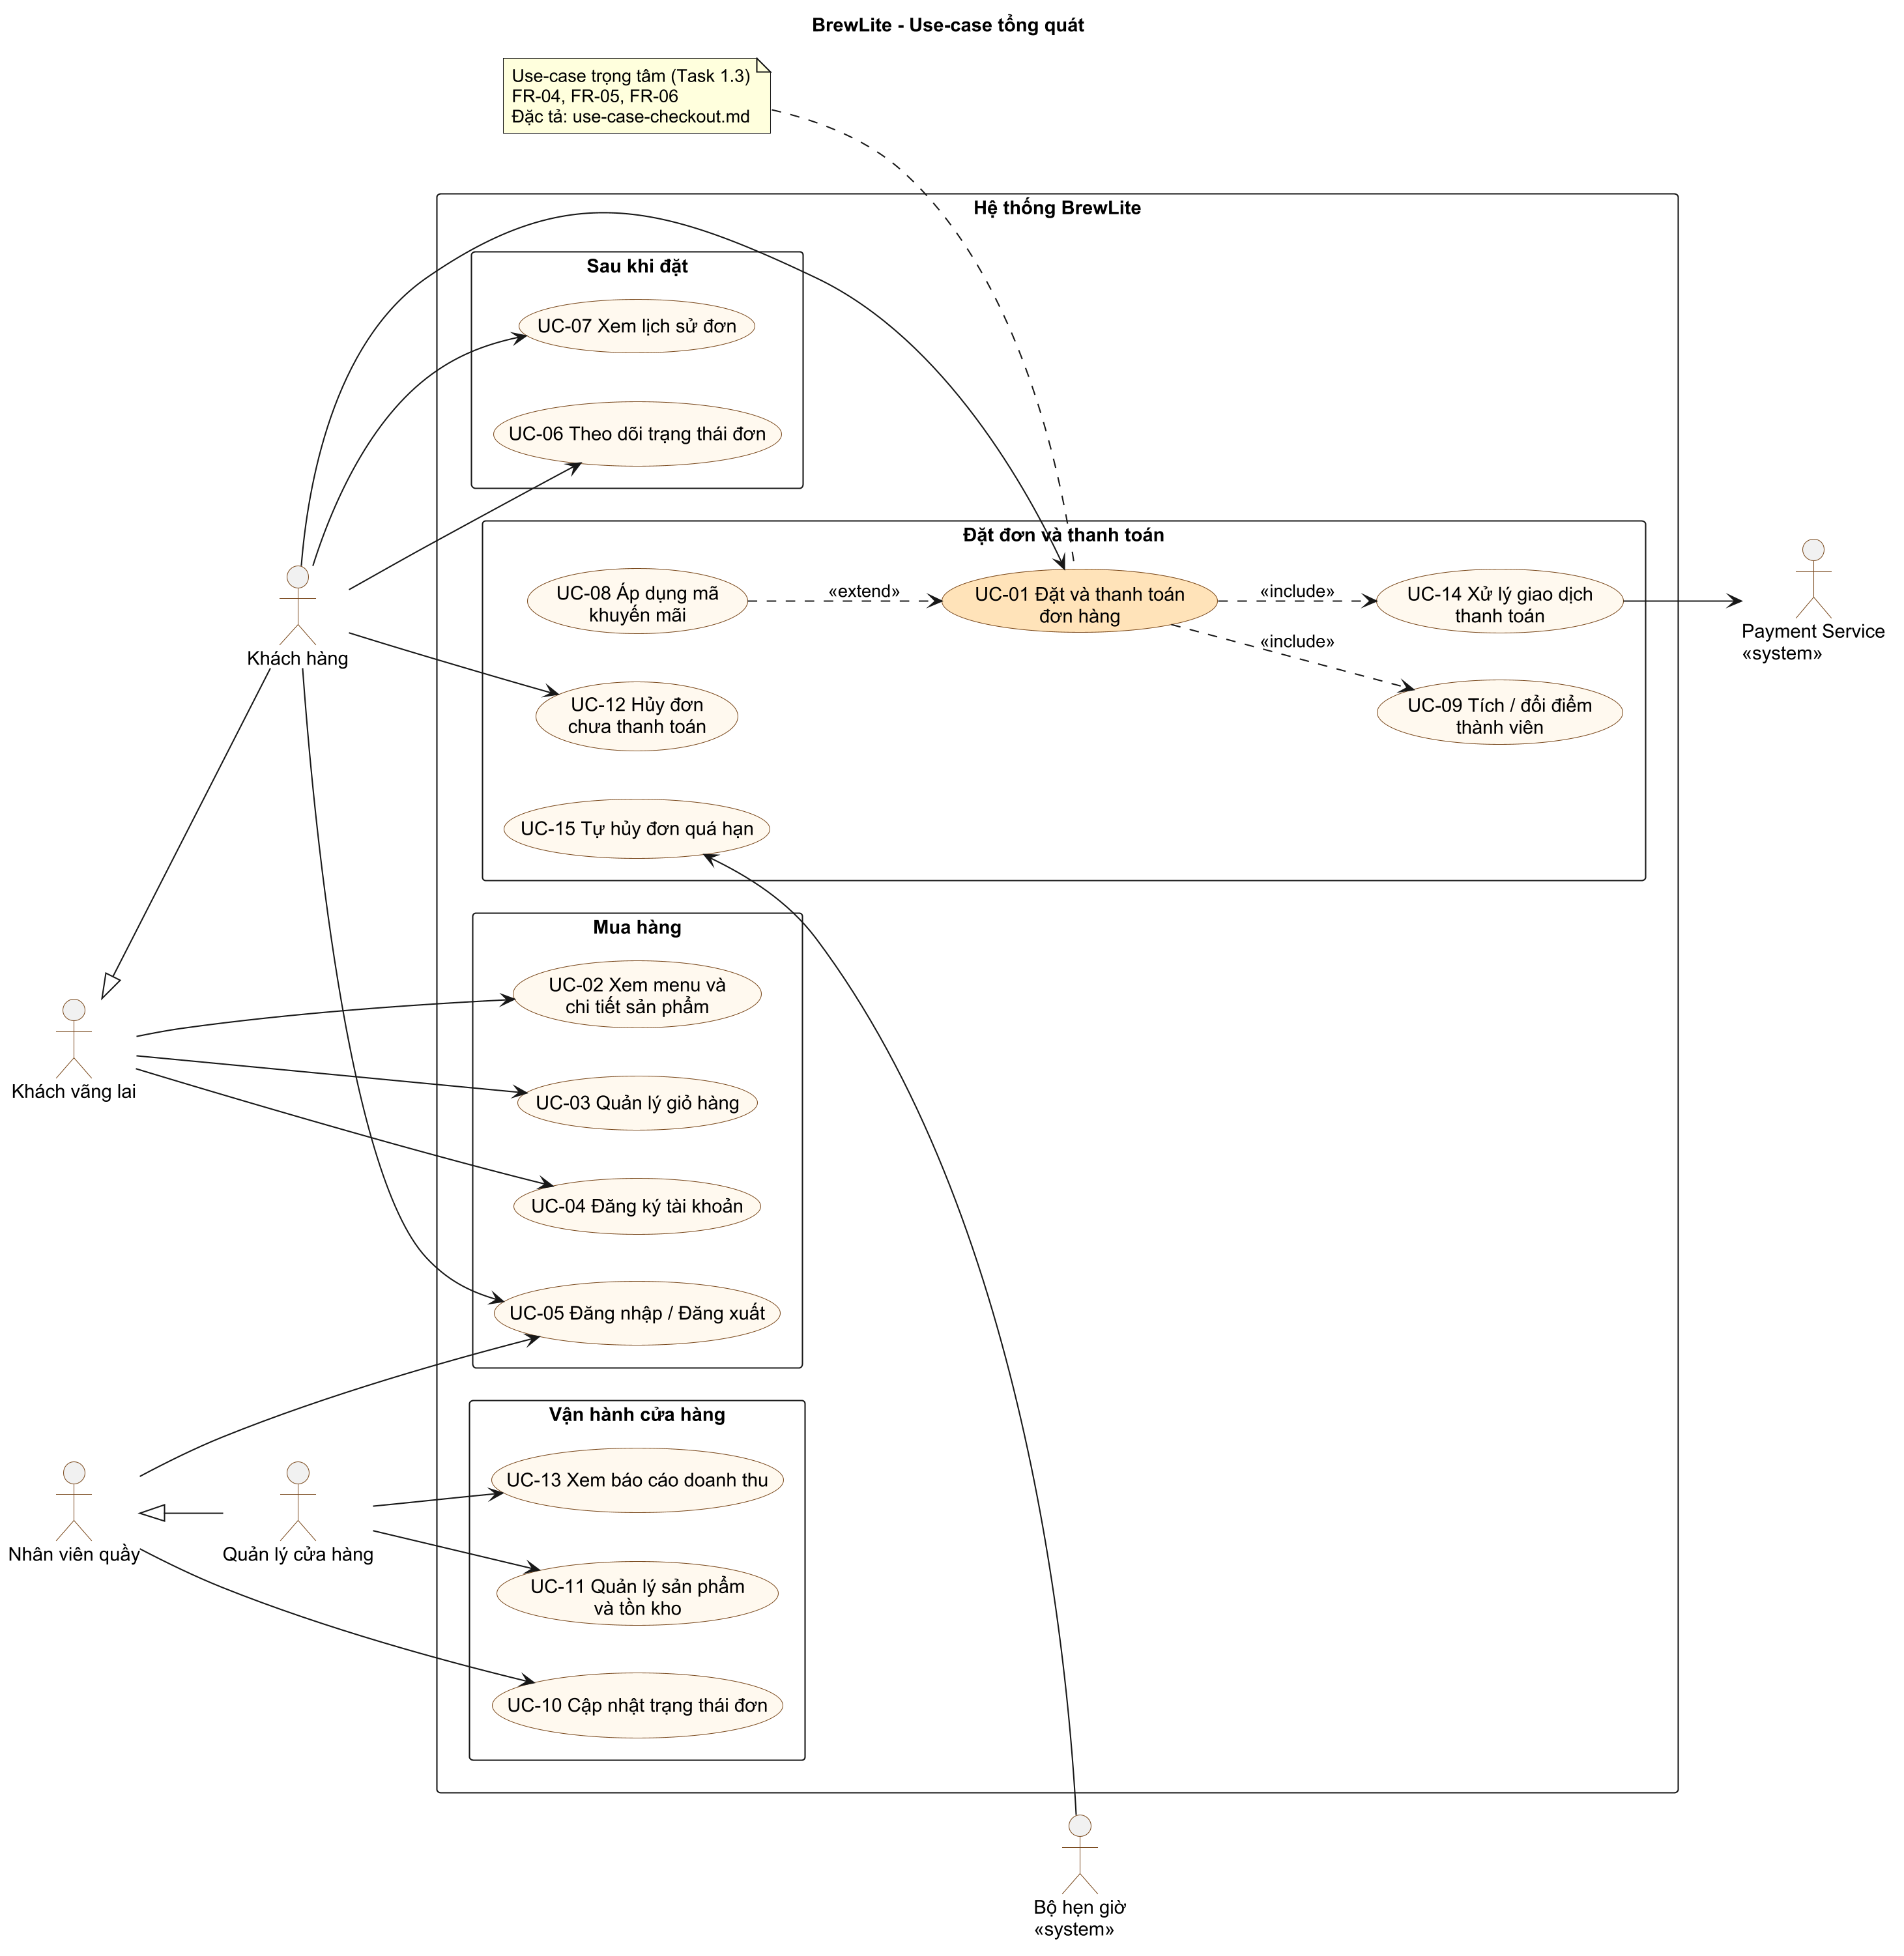
\includegraphics[width=\textwidth,height=0.85\textheight,keepaspectratio]{figures/usecase-overview.png}
\caption{Sơ đồ use-case tổng quát của hệ thống BrewLite}\label{fig:uc-overview}
\end{figure}

\begin{longtable}{|c|p{5.6cm}|p{3.4cm}|p{2.6cm}|c|}
\caption{Danh sách use-case}\label{tab:usecases}\\
\hline
\thead \textbf{Mã} & \textbf{Use-case} & \textbf{Tác nhân chính} & \textbf{Yêu cầu} & \textbf{Ưu tiên} \\ \hline
\endfirsthead
\hline
\thead \textbf{Mã} & \textbf{Use-case} & \textbf{Tác nhân chính} & \textbf{Yêu cầu} & \textbf{Ưu tiên} \\ \hline
\endhead
\textbf{UC-01} & \textbf{Đặt và thanh toán đơn hàng} (trọng tâm) & Khách hàng, Payment Service & FR-04, 05, 06 & Must \\ \hline
UC-02 & Xem menu và chi tiết sản phẩm & Khách vãng lai & FR-01, 02, 17 & Must \\ \hline
UC-03 & Quản lý giỏ hàng & Khách vãng lai & FR-03 & Must \\ \hline
UC-04 & Đăng ký tài khoản & Khách vãng lai & FR-09 & Must \\ \hline
UC-05 & Đăng nhập / Đăng xuất & Khách hàng, Nhân viên, Quản lý & FR-10, 11 & Must \\ \hline
UC-06 & Theo dõi trạng thái đơn & Khách hàng & FR-07, 20 & Must \\ \hline
UC-07 & Xem lịch sử đơn & Khách hàng & FR-08 & Must \\ \hline
UC-08 & Áp dụng mã khuyến mãi (extend UC-01) & Khách hàng & FR-14 & Should \\ \hline
UC-09 & Tích / đổi điểm thành viên & Khách hàng & FR-15, 18 & Should \\ \hline
UC-10 & Cập nhật trạng thái đơn & Nhân viên & FR-12 & Must \\ \hline
UC-11 & Quản lý sản phẩm và tồn kho & Quản lý & FR-16 & Should \\ \hline
UC-12 & Hủy đơn chưa thanh toán & Khách hàng & FR-13 & Should \\ \hline
UC-13 & Xem báo cáo doanh thu & Quản lý & FR-19 & Could \\ \hline
UC-14 & Xử lý giao dịch thanh toán (include của UC-01) & Payment Service & FR-05, 06 & Must \\ \hline
UC-15 & Tự hủy đơn quá hạn & Bộ hẹn giờ & FR-13 & Should \\ \hline
\end{longtable}

\subsubsection{User story}

\begin{longtable}{|c|p{9.4cm}|p{2.2cm}|p{1.8cm}|}
\caption{User story}\label{tab:userstories}\\
\hline
\thead \textbf{Mã} & \textbf{User story} & \textbf{Yêu cầu} & \textbf{UC} \\ \hline
\endfirsthead
\hline
\thead \textbf{Mã} & \textbf{User story} & \textbf{Yêu cầu} & \textbf{UC} \\ \hline
\endhead
US-01 & Là khách, tôi muốn xem menu theo danh mục và tìm món, để chọn đồ uống nhanh. & FR-01, 17 & UC-02 \\ \hline
US-02 & Là khách, tôi muốn chọn size, topping và thấy giá thay đổi ngay, để biết chính xác số tiền. & FR-02 & UC-02 \\ \hline
US-03 & Là khách, tôi muốn thêm, sửa, xóa món trong giỏ và thấy tổng tiền, để kiểm tra trước khi đặt. & FR-03 & UC-03 \\ \hline
US-04 & Là khách, tôi muốn đăng ký và đăng nhập, để đặt đơn và lưu lịch sử. & FR-09, 10 & UC-04, 05 \\ \hline
US-05 & Là khách hàng, tôi muốn đặt đơn và thanh toán bằng ví hoặc thẻ, để không phải xếp hàng. & FR-04, 05, 06 & UC-01 \\ \hline
US-06 & Là khách hàng, tôi muốn biết khi nào đơn sẵn sàng, để ra quầy lấy đúng lúc. & FR-07 & UC-06 \\ \hline
US-07 & Là khách hàng, tôi muốn xem lại các đơn đã đặt, để đặt lại món quen và đối chiếu chi tiêu. & FR-08 & UC-07 \\ \hline
US-08 & Là khách hàng, tôi muốn nhập mã khuyến mãi, để được giảm giá. & FR-14 & UC-08 \\ \hline
US-09 & Là khách hàng, tôi muốn tích điểm sau mỗi đơn, để được ưu đãi khi quay lại. & FR-15, 18 & UC-09 \\ \hline
US-10 & Là nhân viên quầy, tôi muốn thấy đơn đã thanh toán và đổi trạng thái bằng một chạm, để phục vụ nhanh. & FR-12 & UC-10 \\ \hline
US-11 & Là quản lý, tôi muốn cập nhật sản phẩm, giá và tồn kho, để không bán món đã hết. & FR-16 & UC-11 \\ \hline
US-12 & Là khách hàng, tôi muốn hủy đơn chưa thanh toán, để đổi ý mà không giữ kho của quán. & FR-13 & UC-12 \\ \hline
US-13 & Là quản lý, tôi muốn xem doanh thu theo ngày, để đánh giá kinh doanh. & FR-19 & UC-13 \\ \hline
\end{longtable}

\subsubsection{Giao diện ngoài}

\begin{longtable}{|l|p{5.4cm}|p{4.3cm}|p{2.6cm}|}
\caption{Danh sách API dự kiến}\label{tab:api}\\
\hline
\thead \textbf{Method} & \textbf{Endpoint} & \textbf{Quyền} & \textbf{Yêu cầu} \\ \hline
\endfirsthead
\hline
\thead \textbf{Method} & \textbf{Endpoint} & \textbf{Quyền} & \textbf{Yêu cầu} \\ \hline
\endhead
GET & \code{/products} & Công khai & FR-01, 17 \\ \hline
GET & \code{/products/:id} & Công khai & FR-02 \\ \hline
POST & \code{/auth/register} & Công khai & FR-09 \\ \hline
POST & \code{/auth/login} & Công khai & FR-10 \\ \hline
GET & \code{/me}, \code{/me/loyalty} & CUSTOMER & FR-10, 15 \\ \hline
POST & \code{/orders} & CUSTOMER & FR-04, 14 \\ \hline
GET & \code{/orders}, \code{/orders/:id} & Chủ đơn, STAFF, MANAGER & FR-07, 08 \\ \hline
POST & \code{/orders/:id/cancel} & Chủ đơn & FR-13 \\ \hline
POST & \code{/payments} & Chủ đơn & FR-05, 06 \\ \hline
POST & \code{/promotions/validate} & CUSTOMER & FR-14 \\ \hline
GET & \code{/staff/orders} & STAFF, MANAGER & FR-12 \\ \hline
PATCH & \code{/staff/orders/:id/status} & STAFF, MANAGER & FR-12 \\ \hline
POST, PATCH & \code{/manager/products[/:id]} & MANAGER & FR-16 \\ \hline
GET & \code{/manager/reports/daily} & MANAGER & FR-19 \\ \hline
GET & \code{/health} & Công khai & NFR-14 \\ \hline
\end{longtable}

\textbf{Giao diện với Payment Service:} HTTPS/JSON đồng bộ, timeout 10 giây. Yêu cầu \code{POST /charges}
\code{\{amount, currency: VND, method, source, reference\}} kèm header \code{Idempotency-Key}; phản hồi
\code{\{transactionId, status: SUCCEEDED | FAILED, failureCode?\}}. Cùng khóa thì trả cùng kết quả, không tạo
giao dịch mới.

%%%%%%%%%%%%%%%%%%%%%%%%%%%%%%%%%%%%%%%%%%%%%%%%%%%%%%%%%%%%%%%%%%%%%%
\newpage
\subsection{Task 1.3 -- Đặc tả use-case trọng tâm: UC-01 Đặt và thanh toán đơn hàng}\label{sec:uc01}

\textbf{Lý do chọn:} đây là use-case tạo ra doanh thu và đi qua mọi thành phần quan trọng: xác thực, tính giá,
tồn kho, transaction, dịch vụ thanh toán bên ngoài, idempotency và loyalty. Nó là phần lõi của luồng bắt buộc
\textit{Giỏ hàng $\rightarrow$ Đặt đơn $\rightarrow$ Thanh toán $\rightarrow$ Theo dõi đơn}.

\begin{figure}[H]
\centering
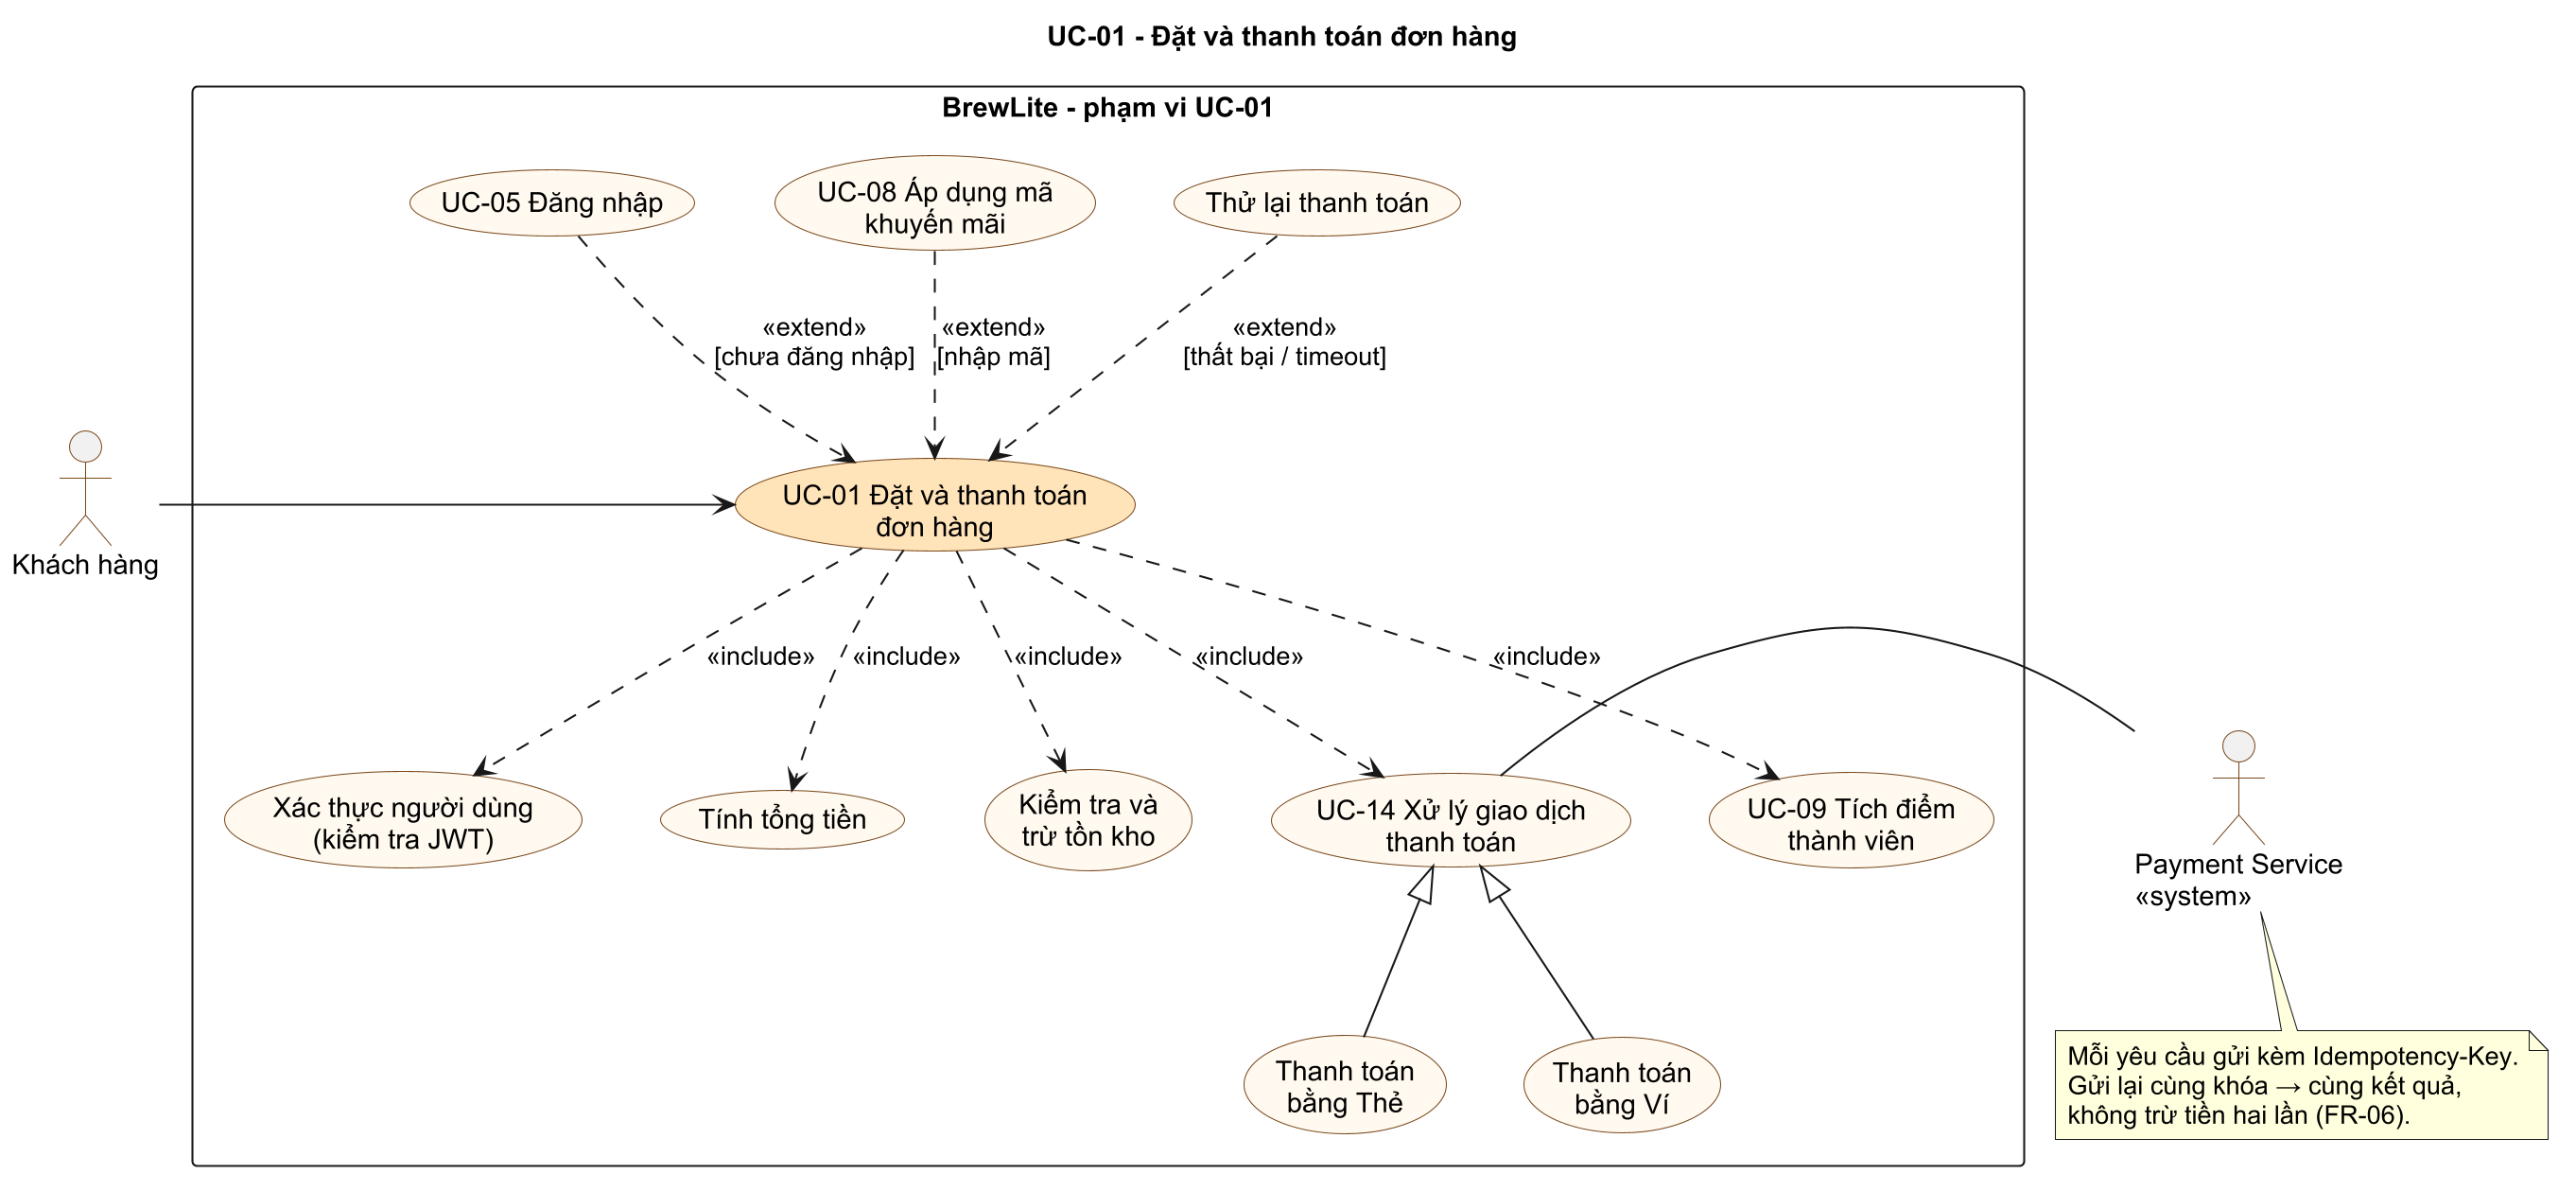
\includegraphics[width=\textwidth]{figures/usecase-checkout.png}
\caption{Use-case diagram cho phạm vi UC-01}\label{fig:uc-checkout}
\end{figure}

\begin{longtable}{|p{3.2cm}|p{12.2cm}|}
\caption{Thông tin chung UC-01}\label{tab:uc01-info}\\
\hline
\thead \textbf{Mục} & \textbf{Nội dung} \\ \hline
\endfirsthead
\hline
\thead \textbf{Mục} & \textbf{Nội dung} \\ \hline
\endhead
Mã / Tên & UC-01 -- Đặt và thanh toán đơn hàng \\ \hline
Mức ưu tiên & Must \\ \hline
Tác nhân chính & Khách hàng (\code{CUSTOMER}) \\ \hline
Tác nhân phụ & Payment Service (hệ thống thanh toán mô phỏng) \\ \hline
Stakeholder và lợi ích & Khách hàng: đặt nhanh, trả đúng tiền, không bị trừ tiền hai lần. Quản lý: không bán vượt kho, ghi nhận doanh thu chính xác. Nhân viên: chỉ nhận đơn đã thanh toán. Đơn vị thanh toán: yêu cầu hợp lệ, có idempotency key. \\ \hline
Trigger & Khách hàng bấm ``Đặt hàng'' trên màn Giỏ hàng (\code{/cart}). \\ \hline
Tiền điều kiện & P1. Giỏ hàng có ít nhất 1 dòng hợp lệ (FR-03). P2. Quán đang hoạt động; API, database sẵn sàng. (Khách chưa đăng nhập vẫn bắt đầu được; xử lý ở luồng A1.) \\ \hline
Hậu điều kiện -- thành công & S1. Có \code{Order} \code{PAID} với mã \code{BL-YYMMDD-NNNN} và snapshot giá. S2. Tồn kho giảm đúng số lượng đặt. S3. Có đúng 1 \code{Payment} \code{SUCCEEDED}, \code{amount = Order.total}, chỉ lưu 4 số cuối thẻ. S4. Có \code{LoyaltyTransaction EARN}. S5. Đơn xuất hiện trên bảng đơn nhân viên. S6. Khách thấy màn xác nhận có số gọi món. S7. Giỏ hàng đã được xóa. \\ \hline
Hậu điều kiện -- thất bại & F1. Không có payment \code{SUCCEEDED}, khách không bị trừ tiền. F2. Đơn chưa tạo thì tồn kho giữ nguyên; đơn đã tạo thì ở \code{PENDING\_PAYMENT} (còn thử lại được) hoặc \code{CANCELLED} và đã hoàn kho. F3. Khách thấy lý do thất bại bằng tiếng Việt. \\ \hline
Yêu cầu liên quan & FR-03, 04, 05, 06, 07, 10, 13, 14, 15; NFR-04, 05, 13; BR-02 $\rightarrow$ BR-11, BR-13, 14, 17, 18 \\ \hline
Tần suất & Cao: khoảng 100--300 đơn/ngày, dồn vào giờ cao điểm \\ \hline
\end{longtable}

\subsubsection{Luồng chính}

\begin{longtable}{|c|p{2.2cm}|p{11.3cm}|}
\caption{Luồng chính UC-01}\label{tab:uc01-main}\\
\hline
\thead \textbf{Bước} & \textbf{Tác nhân} & \textbf{Hành động} \\ \hline
\endfirsthead
\hline
\thead \textbf{Bước} & \textbf{Tác nhân} & \textbf{Hành động} \\ \hline
\endhead
1 & Khách hàng & Ở màn Giỏ hàng, bấm ``Đặt hàng''. \\ \hline
2 & UI & Kiểm tra khách đã đăng nhập và token còn hạn (chưa đăng nhập $\rightarrow$ A1). \\ \hline
3 & UI & Hiện màn Thanh toán: danh sách món, Tạm tính, ô mã khuyến mãi, chọn phương thức Thẻ hoặc Ví. \\ \hline
4 & Khách hàng & Chọn phương thức, nhập thông tin thẻ (số thẻ, hạn, CVV) hoặc ví (SĐT) (nhập mã khuyến mãi $\rightarrow$ A2). \\ \hline
5 & UI & Validate dữ liệu ở client (sai $\rightarrow$ E1). \\ \hline
6 & Khách hàng & Bấm ``Thanh toán''. \\ \hline
7 & UI & Gửi \code{POST /orders} kèm JWT, \code{items}, \code{promoCode?}, \code{expectedTotal}. \\ \hline
8 & API & Xác thực JWT (hết hạn $\rightarrow$ E2), validate body (sai $\rightarrow$ E1). \\ \hline
9 & API & Tính lại giá từ database theo BR-02, BR-04 (lệch giá $\rightarrow$ E3). \\ \hline
10 & API & Mở transaction: kiểm tra và trừ tồn kho từng sản phẩm (không đủ $\rightarrow$ E4); tạo \code{Order} (\code{PENDING\_PAYMENT}, \code{expiresAt} = now + 15 phút) và các \code{OrderItem}; commit. \\ \hline
11 & API & Trả 201 kèm \code{orderId}, \code{code}, \code{total}, \code{expiresAt}. \\ \hline
12 & UI & Xóa giỏ hàng; sinh \code{Idempotency-Key} (UUID v4) cho lần thanh toán. \\ \hline
13 & UI & Gửi \code{POST /payments} kèm JWT, \code{Idempotency-Key}, \code{orderId}, \code{method}, thông tin thẻ/ví. \\ \hline
14 & API & Kiểm tra idempotency key (đã có $\rightarrow$ A3); kiểm tra đơn thuộc khách, đang \code{PENDING\_PAYMENT}, chưa quá hạn (không $\rightarrow$ E5). \\ \hline
15 & API & Tạo \code{Payment} (\code{PENDING}); gọi Payment Service \code{POST /charges} với cùng \code{Idempotency-Key}. \\ \hline
16 & Payment Service & Xử lý giao dịch, trả \code{SUCCEEDED} (thất bại $\rightarrow$ A4; quá 10 giây $\rightarrow$ A5). \\ \hline
17 & API & Một transaction: \code{Payment} $\rightarrow$ \code{SUCCEEDED}; \code{Order} $\rightarrow$ \code{PAID} và ghi lịch sử trạng thái; tăng \code{Promotion.usedCount} (nếu có); tạo \code{LoyaltyTransaction EARN}; lưu response theo idempotency key. \\ \hline
18 & API & Trả 201 \code{\{status: SUCCEEDED, orderStatus: PAID\}}. \\ \hline
19 & UI & Chuyển tới \code{/orders/:id}: ``Thanh toán thành công'', mã đơn, số gọi món, tổng tiền, điểm vừa tích. \\ \hline
20 & Hệ thống & Đơn xuất hiện trên bảng đơn nhân viên ($\le$ 5 giây). Kết thúc use-case. \\ \hline
\end{longtable}

\subsubsection{Luồng thay thế}

\begin{longtable}{|c|p{3.4cm}|p{9.2cm}|p{1.5cm}|}
\caption{Luồng thay thế UC-01}\label{tab:uc01-alt}\\
\hline
\thead \textbf{Mã} & \textbf{Điều kiện} & \textbf{Xử lý} & \textbf{Quay về} \\ \hline
\endfirsthead
\hline
\thead \textbf{Mã} & \textbf{Điều kiện} & \textbf{Xử lý} & \textbf{Quay về} \\ \hline
\endhead
A1 & Chưa đăng nhập hoặc token hết hạn (bước 2) & UI chuyển tới \code{/login?returnUrl=/checkout}, giữ nguyên giỏ; khách đăng nhập (UC-05) hoặc đăng ký (UC-04); thành công thì quay lại \code{/checkout}. Khách hủy đăng nhập thì kết thúc, giỏ vẫn còn. & Bước 3 \\ \hline
A2 & Nhập mã khuyến mãi (bước 4), UC-08 & UI gọi \code{POST /promotions/validate}; hợp lệ thì hiện số tiền giảm và Tổng mới; không hợp lệ thì hiện lý do, khách sửa hoặc bỏ mã. & Bước 4 \\ \hline
A3 & Client gửi lại \code{POST /payments} cùng \code{Idempotency-Key} (bước 14) & API trả đúng response cũ đã lưu, không gọi lại Payment Service. Request trước cùng khóa còn xử lý thì trả 409 \code{REQUEST\_IN\_PROGRESS}, UI chờ 2 giây rồi gửi lại. & Bước 18 \\ \hline
A4 & Payment Service trả \code{FAILED} (bước 16) & Lưu \code{Payment FAILED} kèm mã lỗi; đơn vẫn \code{PENDING\_PAYMENT}, kho vẫn giữ; trả 402; UI hiện lý do, nút ``Thử lại'' và ``Đổi phương thức''; lần thử mới dùng khóa mới. Thất bại lần 3 $\rightarrow$ E6. & Bước 4 \\ \hline
A5 & Payment Service không phản hồi trong 10 giây (bước 16) & Giữ \code{Payment PENDING}, trả 202; UI hiện ``Đang xử lý'' và gửi lại cùng khóa sau 3 giây (tối đa 5 lần); API gọi lại Payment Service cùng khóa và nhận kết quả của giao dịch cũ. & Bước 17 hoặc A4 \\ \hline
A6 & Thanh toán lại một đơn \code{PENDING\_PAYMENT} có sẵn & UI mở \code{/checkout?orderId=...}, bỏ qua bước 7--11. & Bước 12 \\ \hline
\end{longtable}

\subsubsection{Luồng ngoại lệ}

\begin{longtable}{|c|p{3.6cm}|p{5.6cm}|p{4.4cm}|}
\caption{Luồng ngoại lệ UC-01}\label{tab:uc01-exc}\\
\hline
\thead \textbf{Mã} & \textbf{Điều kiện} & \textbf{Xử lý của hệ thống} & \textbf{Kết quả} \\ \hline
\endfirsthead
\hline
\thead \textbf{Mã} & \textbf{Điều kiện} & \textbf{Xử lý của hệ thống} & \textbf{Kết quả} \\ \hline
\endhead
E1 & Dữ liệu không hợp lệ (bước 5, 8) & Client chặn và báo lỗi từng ô; tới server thì trả 400 kèm lỗi từng trường. & Không tạo đơn, không gọi Payment Service; khách sửa và làm lại từ bước 4. \\ \hline
E2 & JWT thiếu, sai hoặc hết hạn (bước 8, 14) & Trả 401. & Chuyển sang A1. \\ \hline
E3 & Giá đã thay đổi (bước 9) & Trả 409 \code{PRICE\_CHANGED} kèm giá mới. & UI cập nhật giỏ, báo giá thay đổi, quay về bước 3. \\ \hline
E4 & \textbf{Hết hàng} (bước 10) & Rollback transaction; trả 409 \code{OUT\_OF\_STOCK} kèm \code{productIds}. & Không tạo đơn, không trừ kho; UI đánh dấu ``Hết hàng'' trên các dòng đó. \\ \hline
E5 & Đơn không còn thanh toán được (bước 14) & Trả 409 \code{ORDER\_ALREADY\_PAID} hoặc \code{ORDER\_NOT\_PAYABLE}. & Đã \code{PAID}: chuyển màn xác nhận. Đã hủy/hết hạn: báo và gợi ý đặt lại. \\ \hline
E6 & Thanh toán thất bại lần thứ 3 & Một transaction: \code{Order CANCELLED}, hoàn kho, ghi lịch sử. & Kết thúc thất bại (F1--F3). \\ \hline
E7 & Đơn quá 15 phút chưa thanh toán & Bộ hẹn giờ (UC-15) hủy đơn và hoàn kho. & Kết thúc thất bại. \\ \hline
E8 & Lỗi hệ thống (500, mất kết nối DB) & Rollback; log lỗi kèm \code{requestId}; trả 500/503 với thông báo chung. & UI báo lỗi, giữ dữ liệu đã nhập; gửi lại thanh toán cùng khóa nên an toàn. \\ \hline
\end{longtable}

\subsubsection{Quy tắc đặc biệt}
\begin{itemize}
  \item Số tiền thanh toán luôn lấy từ \code{Order.total} trên server, không lấy từ client (BR-05, BR-10).
  \item Mỗi đơn có tối đa 1 payment \code{SUCCEEDED}, đảm bảo bằng ràng buộc unique có điều kiện trong database.
  \item Idempotency key hiệu lực 24 giờ, gắn với người dùng (BR-11).
  \item Không lưu số thẻ đầy đủ và CVV (BR-18).
  \item Bước 10 và bước 17 đều là transaction; thất bại giữa chừng không để lại dữ liệu nửa vời (NFR-13).
\end{itemize}

\subsubsection{Liên kết use-case -- yêu cầu -- tiêu chí chấp nhận}

\begin{longtable}{|p{3.6cm}|p{3.8cm}|p{7.4cm}|}
\caption{Liên kết UC-01 với yêu cầu}\label{tab:uc01-trace}\\
\hline
\thead \textbf{Phần của UC-01} & \textbf{Yêu cầu} & \textbf{Tiêu chí chấp nhận dùng để viết test} \\ \hline
\endfirsthead
\hline
\thead \textbf{Phần của UC-01} & \textbf{Yêu cầu} & \textbf{Tiêu chí chấp nhận dùng để viết test} \\ \hline
\endhead
Bước 2, A1, E2 & FR-10, NFR-04 & AC-04.1, AC-10.3, AC-10.5 \\ \hline
Bước 3, A2 & FR-03, FR-14 & AC-03.3, AC-14.1 $\rightarrow$ AC-14.3 \\ \hline
Bước 5, 8, E1 & FR-04, FR-05, NFR-05 & AC-04.2, AC-05.2 \\ \hline
Bước 9, E3 & FR-04 & AC-04.3 \\ \hline
Bước 10--11, E4 & FR-04, NFR-13 & AC-04.4 $\rightarrow$ AC-04.7 \\ \hline
Bước 12--18 & FR-05 & AC-05.1, AC-05.3, AC-05.4, AC-05.8 \\ \hline
A3, A5, E8 & FR-06 & AC-05.7, AC-06.1 $\rightarrow$ AC-06.5 \\ \hline
A4, E6 & FR-05, FR-13 & AC-05.5, AC-05.6 \\ \hline
E5, E7 & FR-05, FR-13 & AC-05.3, AC-06.5, AC-13.3 \\ \hline
Bước 17 & FR-14, FR-15 & AC-14.4, AC-15.1, AC-15.2 \\ \hline
Bước 19--20 & FR-07, FR-12 & AC-07.1, AC-12.2 \\ \hline
\end{longtable}

\subsubsection{Kịch bản kiểm thử nghiệm thu}

\begin{longtable}{|c|p{3.2cm}|p{3.9cm}|p{6.0cm}|}
\caption{Kịch bản nghiệm thu rút từ UC-01}\label{tab:uat}\\
\hline
\thead \textbf{Mã} & \textbf{Kịch bản} & \textbf{Dữ liệu} & \textbf{Kết quả mong đợi} \\ \hline
\endfirsthead
\hline
\thead \textbf{Mã} & \textbf{Kịch bản} & \textbf{Dữ liệu} & \textbf{Kết quả mong đợi} \\ \hline
\endhead
UAT-01 & Luồng chính bằng thẻ & Thẻ \code{4242...4242}, 2 ly & Đơn \code{PAID}, kho $-$2, 1 payment \code{SUCCEEDED}, màn xác nhận có số gọi món \\ \hline
UAT-02 & Luồng chính bằng ví & SĐT \code{0912345678} & Như UAT-01 với phương thức Ví \\ \hline
UAT-03 & Chưa đăng nhập (A1) & Khách vãng lai có giỏ 1 ly & Chuyển đăng nhập, giỏ còn nguyên, quay lại thanh toán \\ \hline
UAT-04 & Hết hàng (E4) & Sản phẩm còn 1, đặt 2 & 409 \code{OUT\_OF\_STOCK}, không có đơn, kho vẫn 1 \\ \hline
UAT-05 & Thẻ bị từ chối (A4) & Thẻ \code{4000...0002} & 402; đơn \code{PENDING\_PAYMENT}; thử lại bằng \code{4242...} thì thành công \\ \hline
UAT-06 & Thất bại 3 lần (E6) & 3 lần thẻ \code{...0002} & Đơn \code{CANCELLED}, kho được hoàn \\ \hline
UAT-07 & Gửi lại cùng khóa (A3) & 2 lần cùng \code{Idempotency-Key} & Cùng response; Payment Service gọi 1 lần; 1 payment \\ \hline
UAT-08 & Timeout (A5) & Thẻ \code{4000...0119} & Lần đầu 202 \code{PENDING}; gửi lại cùng khóa thì \code{SUCCEEDED} \\ \hline
UAT-09 & Mã khuyến mãi (A2) & \code{GIAM10}, Tạm tính 150.000 & Tổng 135.000; \code{usedCount} +1 sau khi \code{PAID} \\ \hline
UAT-10 & Đặt đồng thời & 10 khách cùng đặt 1 ly, kho còn 5 & Đúng 5 đơn thành công, kho = 0 \\ \hline
\end{longtable}
